\documentclass[conference]{IEEEtran}

\usepackage{graphicx}
\graphicspath{{images/}}

\usepackage{amsmath}
\usepackage{amssymb}
\usepackage{cite}
\usepackage{booktabs}
\usepackage{array}
\usepackage{url}
\usepackage[hidelinks]{hyperref}

% Packages for better tables
\usepackage{array}
\usepackage{tabularx}
\usepackage{graphicx}
\usepackage{makecell}

\renewcommand{\arraystretch}{1.2}

\begin{document}

\title{An Intelligent Weather Monitoring System Using IoT Sensors, Predictive Modeling, and Power BI Reporting}

\author{

\IEEEauthorblockN{
\href{mailto:nayansaha636@gmail.com}{Nayan Saha},
\href{mailto:bani.manna4509@gmail.com}{Banibrata Manna},
\href{mailto:mrinmayeemaiti@gmail.com}{Mrinmayee Maity},
\href{mailto:sunayanimondal1403@gmail.com}{Sunayani Mondal},
\href{mailto:chhotan1419@gmail.com}{Chhotan Mal},
\href{mailto:debayan@gcelt.gov.in}{Debayan Ganguly}
}

\IEEEauthorblockA{
Department of Computer Science and Engineering\\
Government College of Engineering and Leather Technology\\
Kolkata, India
}

}

\maketitle

\begin{abstract}

This paper presents an IoT-based intelligent weather monitoring system integrated with Machine Learning (ML) techniques for environmental prediction and analysis. The proposed system utilizes an Arduino UNO R4 WiFi board to collect real-time environmental data through multiple sensors, including DHT11, BMP280, MQ-135, LDR and rain sensors.

The acquired data are transmitted to the ThingSpeak cloud platform for storage, visualization, and further analysis. Machine Learning models such as Random Forest and XGBoost are used to predict weather conditions and the air quality index (AQI). A Flask-based web application and a Power BI dashboard have been developed to visualize both real-time and predicted environmental parameters. Experimental results demonstrate the effectiveness of the proposed framework in delivering accurate weather monitoring and predictive analytics while maintaining a lightweight and cost-effective architecture.

\end{abstract}

\begin{IEEEkeywords}
Internet of Things (IoT), Machine Learning, Weather Forecasting, Arduino UNO R4 WiFi, ThingSpeak, Power BI, Air Quality Index (AQI)
\end{IEEEkeywords}

\section{Introduction}

Weather forecasting plays a vital role in many areas such as agriculture, transportation, and disaster response [1]. Classical approaches based on meteorological stations are unable to account for hyper-local climate conditions. The emergence of IoT technology makes it possible to use the concept of distributed sensor networks, which can monitor environmental conditions in real time [2].

At the same time, ML approaches are able to process multidimensional meteorological information more efficiently than classical statistical ones [3]. This combination can help achieve accurate weather observation and short-range forecasting.

The project introduces a smart weather station, which is going to monitor temperature, humidity, atmospheric pressure, precipitation, light intensity, and air quality. Processing is performed by the Arduino UNO R4 WiFi. Data will be visualized locally with the OLED display and sent to the cloud for further processing and visualization with ML and Power BI.

\section{Literature Review}

Current advancements in weather monitoring depend on the utilization of IoT and ML to enhance the current methods used. A range of research papers [1]-[9] has investigated ways of acquiring real-time data, increasing forecasting accuracy, and improving coverage. Earlier investigations relied on using machine learning techniques to perform weather forecasts based on historical information.

For example, deep learning algorithms such as LSTM and GRU have proven effective in forecasting future changes in temperatures and air quality using time series [1].

Alternatively, regression models such as SVR could also be applied to produce forecasts but had poor results because they are not efficient when dealing with highly nonlinear environmental data [9].

By integrating IoT technology, scientists introduced methods of real-time data collection based on sensors into their weather monitoring techniques. One such IoT-based system relies on utilizing various sensors, namely DHT11, BMP280, and MQ135, to gather information about temperature, humidity, atmospheric pressure, and air quality [6]. Although the above systems are efficient in collecting real-time data, they are still unable to produce analyses or make predictions.

The integration of IoT and ML is increasingly becoming popular in recent literature. The combination of the two was applied to create an IoT-based weather monitoring and forecasting application using the Random Forest algorithm, which enhanced the accuracy of temperature prediction [2]. Other configurations of IoT and ML could also be used to predict rainfall with fair accuracy [3].

Most recently, distributed hyperlocal weather prediction systems combining IoT and ML were suggested [5]. Air Quality Index (AQI) prediction has also gained attention due to increasing environmental concerns. 

Hybrid deep learning models and ensemble techniques such as XGBoost have demonstrated strong performance in AQI classification tasks, achieving higher accuracy compared to traditional models [8].

Author proposed a low-cost, energy-efficient IoT-assisted wireless sensor network for soil moisture measurement using neural network models in the context of soil information prediction. To use water as efficiently as possible, to investigate a smart irrigation system incorporating LoRa[10] technology with deep learning. Advanced soil moisture prediction was achieved using machine learning approaches.

Comparative analysis of the above literature reveals that even though deep learning models exhibit high prediction accuracies, they are not suitable for real-time implementation. On the other hand, IoT models have the potential for real-time monitoring but cannot yield high predictive accuracies as no adequate modeling process can be applied. Moreover, all the available studies have concentrated on developing prediction models on a single parameter, such as temperature or rainfall.

In this case, the presented work stands out because it incorporates IoT-enabled real-time data acquisition capabilities and employs multi-parameter machine learning models for making predictions based on temperature forecast, rain prediction, and AQI classification. The difference between the proposed work and the available literature is that the presented study uses different machine learning models, including Random Forest and XGBoost, and carries out a comparative analysis of their performances. For instance, the temperature forecast model yielded a high accuracy (R² = 0.94), while rain prediction reached a classification accuracy of 100\%, surpassing many existing solutions.

Besides, the proposed model has incorporated ThingSpeak cloud integration, Power BI, and web application development using Flask. In essence, there is no other study where such an effort has been made.

To sum up, this work not only increases the prediction accuracy but also adds a dimension to the practical implementation of the whole system.

\section{System Architecture}

The proposed architecture consists of three primary layers:

\begin{itemize}
\item Sensing Layer
\item Processing and Communication Layer
\item Application and Analytics Layer
\end{itemize}

\begin{figure}[!t]
\centering
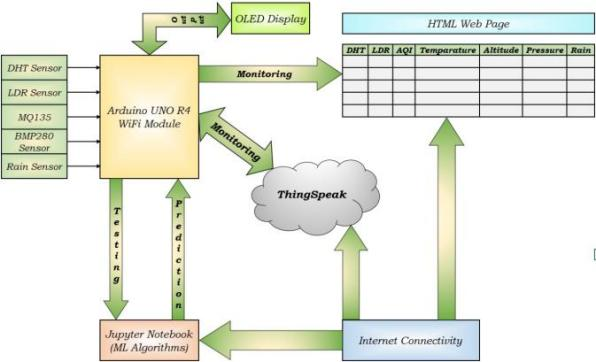
\includegraphics[width=\columnwidth]{image_1.jpeg}
\caption{Overall System Architecture}
\label{fig:system_architecture}
\end{figure}

The sensing layer collects environmental data using multiple sensors. The processing layer performs local data acquisition and cloud transmission through the Arduino UNO R4 WiFi platform. The application layer includes ThingSpeak, Machine Learning models, Power BI dashboards, and a Flask-based web application for visualization and prediction.

\subsection{Hardware Components}

The proposed weather monitoring system integrates multiple sensors and embedded devices to acquire environmental parameters in real time. Each component contributes to measuring specific atmospheric conditions required for monitoring and prediction.

\subsubsection{Arduino UNO R4 WiFi}

The Arduino UNO R4 WiFi serves as the central processing unit of the system. It features a 32-bit Renesas RA4M1 microcontroller and an ESP32-S3 coprocessor that provides wireless connectivity. The board is responsible for collecting sensor readings, processing data, displaying measurements on the OLED display, and transmitting information to the ThingSpeak cloud platform.

\begin{figure}[!t]
\centering
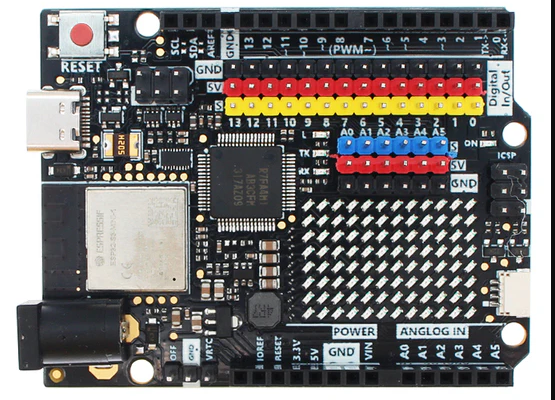
\includegraphics[width=0.8\columnwidth]{image_9.png}
\caption{Arduino UNO R4 WiFi}
\label{fig:arduino}
\end{figure}

\subsubsection{DHT11 Sensor}

The DHT11 sensor measures ambient temperature and relative humidity. It is widely used in environmental monitoring applications due to its simplicity, low cost, and ease of integration with microcontrollers.

\begin{figure}[!t]
\centering
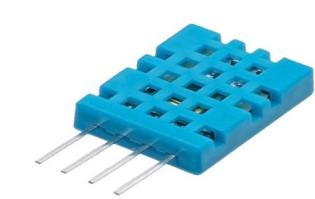
\includegraphics[width=0.7\columnwidth]{image_10.jpeg}
\caption{DHT11 Temperature and Humidity Sensor}
\label{fig:dht11}
\end{figure}

\subsubsection{BMP280 Sensor}

The BMP280 is a high-precision digital sensor used for measuring atmospheric pressure and estimating altitude. The sensor provides reliable pressure readings, which are valuable for weather forecasting applications.

\begin{figure}[!t]
\centering
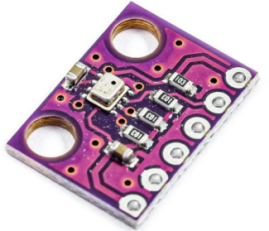
\includegraphics[width=0.7\columnwidth]{image_11.png}
\caption{BMP280 Pressure Sensor}
\label{fig:bmp280}
\end{figure}

\subsubsection{MQ-135 Sensor}

The MQ-135 sensor is utilized to monitor air quality by detecting gases such as carbon dioxide (CO$_2$), ammonia (NH$_3$), benzene, smoke, and other pollutants. The collected measurements are used for Air Quality Index prediction.

\begin{figure}[!t]
\centering
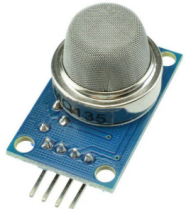
\includegraphics[width=0.7\columnwidth]{image_12.png}
\caption{MQ-135 Air Quality Sensor}
\label{fig:mq135}
\end{figure}

\subsubsection{Rain Sensor}

The rain sensor detects the presence and intensity of rainfall using a conductive sensing plate. The measured values are used both for monitoring and rainfall prediction.

\begin{figure}[!t]
\centering
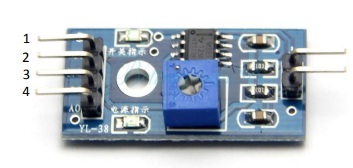
\includegraphics[width=0.7\columnwidth]{image_13.jpeg}
\caption{Rain Detection Sensor}
\label{fig:rainsensor}
\end{figure}

\subsubsection{LDR Sensor}

The Light Dependent Resistor (LDR) measures ambient light intensity and assists in identifying day-night environmental conditions.

\begin{figure}[!t]
\centering
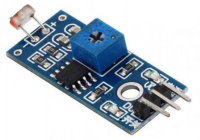
\includegraphics[width=0.7\columnwidth]{image_14.png}
\caption{Light Dependent Resistor (LDR)}
\label{fig:ldr}
\end{figure}

\subsubsection{OLED Display}

The OLED display provides immediate on-site visualization of environmental parameters measured by the sensor network.

\begin{figure}[!t]
\centering
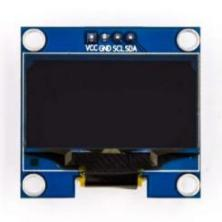
\includegraphics[width=0.7\columnwidth]{image_15.jpeg}
\caption{OLED Display Module}
\label{fig:oled}
\end{figure}

\subsection{Software Components}

The software infrastructure consists of multiple platforms and frameworks working together to support data acquisition, storage, analysis, prediction, and visualization.

\begin{itemize}
\item Arduino IDE
\item ThingSpeak Cloud Platform
\item Python Programming Language
\item Scikit-Learn Library
\item XGBoost Framework
\item Flask Web Framework
\item Microsoft Power BI
\end{itemize}

Arduino IDE is used for firmware development and sensor integration. ThingSpeak serves as the cloud platform for data storage and real-time visualization. Python is employed for data preprocessing, feature engineering, model training, and evaluation.

Scikit-Learn provides implementations of classical Machine Learning algorithms, while XGBoost is utilized for ensemble learning and classification tasks. Flask is used to develop a lightweight web interface for displaying predictions and sensor data. Microsoft Power BI provides interactive dashboards for advanced analytics and decision support.

\subsection{System Implementation}

The proposed weather monitoring and forecasting system consists of multiple environmental sensors interfaced with an Arduino Uno R4 WiFi microcontroller. The sensors continuously monitor various atmospheric parameters, including temperature, humidity, air quality, light intensity, atmospheric pressure, altitude, and rainfall. The LDR, MQ-135, and Rain Sensor are connected to the analog input pins of the microcontroller, while the remaining sensors communicate through digital I/O interfaces. The complete system architecture is illustrated in Fig.~8.

\subsubsection{Environmental Data Acquisition}

The system employs a network of sensors to continuously collect environmental data:

\begin{itemize}
\item \textbf{Temperature and Humidity Monitoring:} The DHT11 sensor measures ambient temperature and relative humidity.

\item \textbf{Air Quality Monitoring:} The MQ-135 gas sensor detects harmful gases such as ammonia, smoke, and other pollutants, enabling the assessment of air quality levels.

\item \textbf{Light Intensity Measurement:} A Light Dependent Resistor (LDR) is used to measure the intensity of sunlight and ambient illumination.

\item \textbf{Atmospheric Pressure and Altitude Measurement:} The BMP280 sensor measures atmospheric pressure and estimates altitude based on pressure variations.

\item \textbf{Rainfall Detection:} The rain sensor detects the presence of moisture on its sensing surface and indicates rainfall conditions.
```

\end{itemize}

\subsubsection{Data Processing and Transmission}

The Arduino Uno R4 WiFi serves as the central processing unit of the system. It collects raw sensor readings and converts them into meaningful physical parameters, such as temperature in degrees Celsius, relative humidity in percentage, atmospheric pressure in hectopascals (hPa), and air quality indicators.

After processing, the microcontroller transmits the sensor data to the ThingSpeak cloud platform using its integrated WiFi module. This enables remote monitoring and long-term storage of environmental information.

\subsubsection{Cloud Storage and Data Visualization}

ThingSpeak functions as a cloud-based data repository, storing all sensor measurements for future analysis. The collected data can be visualized in real time through multiple interfaces:

\begin{itemize}
\item \textbf{OLED Display:} An OLED display connected to the device provides instant visualization of current sensor readings.

```
\item \textbf{Web Dashboard and Power BI:} Sensor data can be displayed through a web application or Power BI dashboard using interactive charts and graphs. These visualizations help identify trends, seasonal variations, and anomalies in environmental conditions over time.
```

\end{itemize}

\subsubsection{Machine Learning-Based Weather Forecasting}

In addition to real-time monitoring, the system incorporates machine learning techniques to improve weather forecasting accuracy. Historical environmental data stored in the cloud is utilized to train predictive models capable of identifying patterns and relationships among different weather parameters.

The forecasting process consists of the following stages:

\begin{itemize}
\item \textbf{Learning:} The system continuously accumulates historical weather data, including temperature, humidity, pressure, rainfall, and air quality measurements. This growing dataset enables the machine learning models to learn long-term environmental patterns and trends.

```
\item \textbf{Prediction:} Machine learning algorithms such as Random Forest and Linear Regression are employed to analyze historical data and generate forecasts. These models can predict future weather conditions, including rainfall probability, temperature trends, humidity levels, and air quality indices.

\item \textbf{Continuous Improvement:} As additional sensor data is collected and stored, the forecasting models are periodically updated, leading to improved prediction accuracy over time.
```

\end{itemize}

Thus, the proposed system integrates IoT-based environmental sensing, cloud computing, real-time visualization, and machine learning techniques to provide a comprehensive solution for weather monitoring and forecasting.


\begin{figure}[!t]
\centering
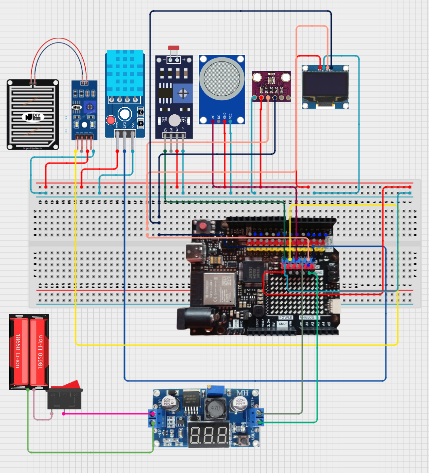
\includegraphics[width=\columnwidth]{image_2.png}
\caption{Complete IoT Weather Monitoring System}
\label{fig:complete_system}
\end{figure}

\begin{figure}[!t]
\centering
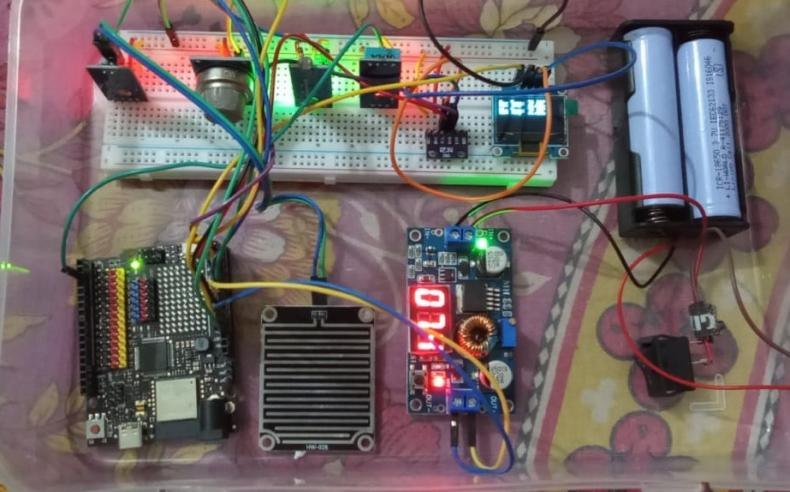
\includegraphics[width=\columnwidth]{image_3.jpeg}
\caption{Hardware Setup and Sensor Integration}
\label{fig:hardware_setup}
\end{figure}

\section{Methodology}

The proposed methodology consists of six major stages:

\begin{enumerate}
\item Data Acquisition
\item Cloud Storage
\item Data Preprocessing
\item Machine Learning Model Development
\item Prediction and Classification
\item Visualization and Reporting
\end{enumerate}

\subsection{Data Acquisition}

Environmental parameters including temperature, humidity, atmospheric pressure, rainfall, air quality, and light intensity are collected through the deployed sensor network.

The Arduino UNO R4 WiFi acquires sensor readings at predefined intervals and transmits the collected data to the ThingSpeak cloud server through HTTP-based communication.

\subsection{Data Storage and Preprocessing}

Sensor readings are stored in dedicated ThingSpeak channels. Historical records are exported as CSV datasets for offline analysis and Machine Learning model development.

The preprocessing pipeline includes:

\begin{itemize}
\item Missing-value handling
\item Data cleaning
\item Feature selection
\item Feature scaling
\item Label encoding
\item Training-testing dataset splitting
\end{itemize}

These steps improve data quality and enhance model performance.

\subsection{Machine Learning Models}

Several Machine Learning algorithms were evaluated for prediction tasks:

\begin{itemize}
\item Random Forest Regressor
\item XGBoost Regressor
\item Decision Tree Classifier
\item Random Forest Classifier
\item Support Vector Machine (SVM)
\item Logistic Regression
\end{itemize}

Temperature forecasting is formulated as a regression problem, whereas rainfall prediction and AQI estimation are treated as classification problems.

\subsection{Visualization Framework}

A Flask-based web application and Microsoft Power BI dashboard are utilized to visualize both real-time sensor measurements and predictive analytics results.

\begin{figure}[!t]
\centering
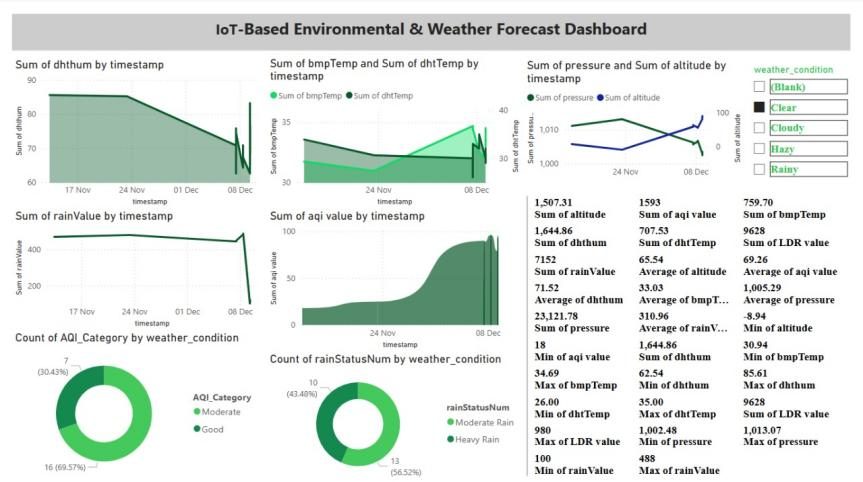
\includegraphics[width=\columnwidth]{image_4.jpeg}
\caption{Power BI Weather Intelligence Dashboard}
\label{fig:powerbi_dashboard}
\end{figure}

\section{Results and Discussion}

\subsection{Sensor Data Analysis}

The proposed IoT-based weather monitoring system successfully collected real-time environmental data, including temperature, humidity, atmospheric pressure, rainfall, light intensity, and air quality measurements. Continuous monitoring revealed clear diurnal variations in temperature and humidity throughout the observation period. Furthermore, the MQ-135 sensor effectively detected changes in air quality, where a decrease in sensor resistance corresponded to increased concentrations of smoke and harmful gases, resulting in higher Air Quality Index (AQI) values.

\subsection{Temperature Forecasting}

Temperature forecasting was performed using Linear Regression, Random Forest, and XGBoost regression models. The performance comparison is presented in Table~\ref{tab:temp_forecast}. Among the evaluated models, Random Forest achieved the highest prediction accuracy with an $R^2$ score of 0.9423 and the lowest Mean Squared Error (MSE) of 5.4177. XGBoost also demonstrated strong predictive capability, whereas Linear Regression exhibited comparatively lower performance.

\begin{table}[ht]
\centering
\caption{Temperature Forecasting Model Performance}
\footnotesize
\begin{tabular}{|p{2.3cm}|p{2.8cm}|p{2.2cm}|}
\hline
\textbf{Model} & \textbf{MSE} & \textbf{R2 Score} \\
\hline
Linear Regression &
29.94449568818 &
0.68114240359 \\
\hline
Random Forest &
5.41769868470 &
0.94231078731 \\
\hline
XGBoost &
9.16129938564 &
0.90244785110 \\
\hline
\end{tabular}
\label{tab:temp_forecast}
\end{table}

The results indicate that ensemble learning methods outperform traditional linear models in capturing nonlinear weather patterns and environmental dependencies.

\subsection{Rainfall Prediction}

Rainfall prediction was formulated as a binary classification problem (Rain/No Rain). Various machine learning classifiers were evaluated using accuracy, precision, recall, and F1-score metrics. The results are summarized in Table~\ref{tab:rain_prediction}.

Random Forest and Decision Tree classifiers achieved perfect classification performance, obtaining 100\% accuracy, precision, recall, and F1-score. Logistic Regression, KNN, and SVM also demonstrated excellent predictive capabilities, achieving accuracies greater than 96\%.

\begin{table}[ht]
\centering
\caption{Rain Forecasting Model Performance}
\label{tab:rain_prediction}
\footnotesize
\begin{tabular}{|p{1.9cm}|c|c|c|c|}
\hline
\textbf{Model} &
\textbf{Accuracy} &
\textbf{Precision} &
\textbf{Recall} &
\textbf{F1-Score} \\
\hline

Logistic Reg. & 0.976 & 0.9925 & 0.9779 & 0.9851 \\
\hline
Decision Tree & 1 & 1 & 1 & 1 \\
\hline
Random Forest & 1 & 1 & 1 & 1 \\
\hline
KNN & 0.9768 & 0.9852 & 0.9852 & 0.9852 \\
\hline
SVM & 0.965 & 0.9710 & 0.9852 & 0.9781 \\
\hline
\end{tabular}
\label{tab:rain_forecast}
\end{table}

These results demonstrate the effectiveness of tree-based ensemble learning methods for rainfall prediction using environmental sensor data.

\subsection{AQI Forecasting}

AQI forecasting was evaluated using multiple regression algorithms. Figure~\ref{fig:aqi_pred} presents the comparison between actual and predicted AQI values generated by the Random Forest Regressor. The quantitative performance metrics are presented in Table~\ref{tab:aqi_forecast}.

\begin{figure}[ht]
\centering
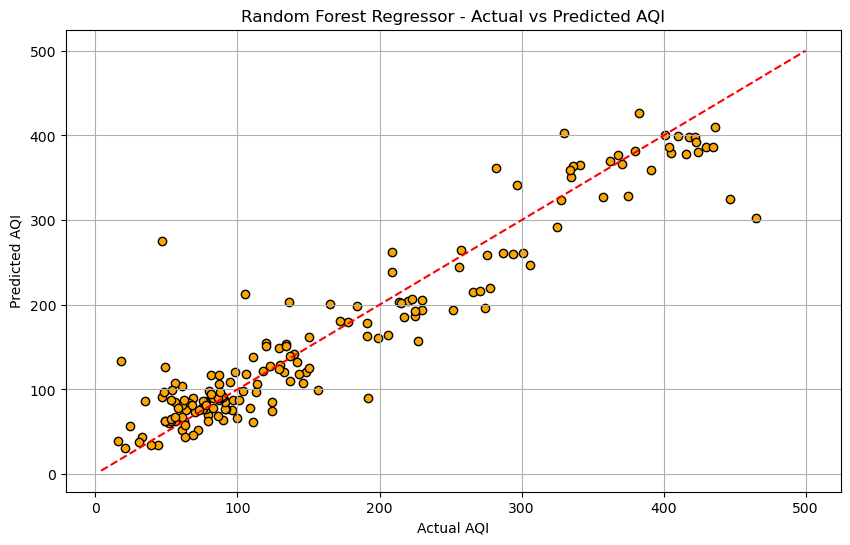
\includegraphics[width=\columnwidth]{image_5.png}
\caption{Random Forest Regressor: Actual vs. Predicted AQI}
\label{fig:aqi_pred}
\end{figure}

Among the models evaluated, Random Forest achieved the best forecast performance with a $R^2$ score of 0.8933 and the lowest MSE of 1564.08. XGBoost closely followed with a $R^2$ score of 0.8655.

\begin{table}[ht]
\centering
\caption{AQI Forecasting Model Performance}
\label{tab:aqi_class}
\footnotesize
\begin{tabular}{|p{2.1cm}|p{2.5cm}|p{2.2cm}|}
\hline
\textbf{Model} & \textbf{MSE} & \textbf{R2 Score} \\
\hline
Linear Regression &
10464.45522217116 &
0.28585394887 \\
\hline
Decision Tree &
4359.45086705202 &
0.70248956532 \\
\hline
Random Forest &
1564.07644797688 &
0.89325970676 \\
\hline
XGBoost &
1970.52890083626 &
0.86552138613 \\
\hline
SVR &
3673.52064475154 &
0.74930082776 \\
\hline
\end{tabular}
\label{tab:aqi_forecast}
\end{table}

The superior performance of Random Forest highlights its ability to model complex interactions among environmental variables affecting air quality.

\subsection{Weather Condition Classification}

Weather conditions were classified into four categories: Clear, Cloudy, Hazy, and Rainy. Random Forest, SVM, and Naive Bayes classifiers were evaluated. The overall classification performance is presented in Table~\ref{tab:weather_perf}, while class-wise F1-scores are summarized in Table~\ref{tab:weather_f1}.

Random Forest achieved perfect classification performance with an overall accuracy of 100\%, whereas SVM and Naive Bayes achieved accuracies of 97.69\% and 97.11\%, respectively.

\begin{table}[ht]
\centering
\caption{Weather Condition Classification Model Comparison}
\label{tab:weather_perf}
\footnotesize
\begin{tabular}{|p{2.3cm}|c|c|c|}
\hline
\textbf{Metric} &
\textbf{Random Forest} &
\textbf{SVM} &
\textbf{Naive Bayes} \\
\hline
Overall Accuracy &
1 &
0.9769 &
0.9711 \\
\hline
Weighted Precision &
1 &
0.97 &
0.98 \\
\hline
Weighted Recall &
1 &
0.98 &
0.97 \\
\hline
Weighted F1-score &
1 &
0.97 &
0.97 \\
\hline
\end{tabular}
\label{tab:weather_classification}
\end{table}

\begin{table}[ht]
\centering
\caption{Class-Wise Performance (F1-Score)}
\footnotesize
\begin{tabular}{|l|c|c|c|}
\hline
\textbf{Weather Class} &
\textbf{Random Forest} &
\textbf{SVM} &
\textbf{Naive Bayes} \\
\hline
Clear & 1 & 0.5 & 0.73 \\
\hline
Cloudy & 1 & 0.95 & 0.87 \\
\hline
Hazy & 1 & 0.92 & 0.78 \\
\hline
Rainy & 1 & 1 & 1 \\
\hline
\end{tabular}
\label{tab:weather_f1}
\end{table}

The class-wise analysis further demonstrates the robustness of the Random Forest classifier, which consistently achieved perfect performance across all weather categories.

\subsection{AQI Category Classification}

AQI values were categorized into standard air-quality classes such as Good, Moderate, and Unhealthy. XGBoost, Decision Tree, and Logistic Regression classifiers were evaluated. The comparative results are presented in Table~\ref{tab:aqi_class}.

XGBoost achieved the highest overall accuracy of 71.43\%, along with the best weighted F1-score, macro-average precision, and macro-average recall values.

\begin{table}[ht]
\centering
\caption{AQI Category Classification Performance}
\footnotesize
\begin{tabular}{|p{2.4cm}|c|c|c|}
\hline
\textbf{Metric} &
\textbf{XGBoost} &
\textbf{Decision Tree} &
\textbf{Logistic Reg.} \\
\hline
Accuracy &
0.7143 &
0.6071 &
0.5119 \\
\hline
Weighted F1-Score &
0.71 &
0.59 &
0.51 \\
\hline
Macro Avg Precision &
0.66 &
0.51 &
0.39 \\
\hline
Macro Avg Recall &
0.65 &
0.51 &
0.34 \\
\hline
\end{tabular}
\label{tab:aqi_category}
\end{table}

The results indicate that boosting-based ensemble methods are particularly effective for multi-class AQI classification tasks involving complex environmental datasets.

\section{Comparison with Existing Systems}

Existing smart environmental monitoring solutions generally focus on either IoT-based data acquisition or machine learning-based prediction. IoT systems provide real-time environmental monitoring using sensors such as DHT11, BMP280, and MQ135, but often lack advanced predictive analytics. In contrast, machine learning and deep learning approaches, including LSTM and GRU models, achieve high forecasting accuracy but typically rely on historical datasets and do not incorporate real-time IoT integration.

Recent studies have attempted to combine IoT platforms with machine learning techniques; however, many remain limited in terms of multi-parameter forecasting, model comparison, scalability, and visualization capabilities. The proposed framework addresses these limitations by integrating real-time IoT sensing, ThingSpeak cloud storage, machine learning-based prediction, Power BI visualization, and Flask-based web deployment into a unified architecture.

Table~\ref{tab:comparison} compares the proposed system with representative approaches reported in the literature.

\begin{table*}[!t]
\centering
\caption{Comparison with Existing IoT-ML Weather Monitoring Systems}
\label{tab:comparison}

\scriptsize
\renewcommand{\arraystretch}{1.15}

\begin{tabular}{|p{3.8cm}|p{2.5cm}|p{2.5cm}|p{2.8cm}|p{2.5cm}|}
\hline
\textbf{Feature} &
\centering\textbf{DL Model \cite{ref1}}\arraybackslash &
\centering\textbf{IoT+ML \cite{ref2}}\arraybackslash &
\centering\textbf{Integrated System \cite{ref3}}\arraybackslash &
\centering\textbf{Proposed System}\arraybackslash \\
\hline

Real-Time IoT Data &
\centering No &
\centering Yes &
\centering Yes &
\centering Yes \arraybackslash \\
\hline

Sensor Integration &
\centering No &
\centering Limited &
\centering Yes &
\centering Multiple Sensors \arraybackslash \\
\hline

Temperature Prediction &
\centering High &
\centering High &
\centering Moderate &
\centering $R^2 = 0.94$ \arraybackslash \\
\hline

Rainfall Prediction &
\centering High &
\centering High &
\centering Moderate &
\centering 100\% Accuracy \arraybackslash \\
\hline

AQI Classification &
\centering High &
\centering Moderate &
\centering Moderate &
\centering 71.43\% Accuracy \arraybackslash \\
\hline

Multi-Parameter Prediction &
\centering No &
\centering No &
\centering Partial &
\centering Yes \arraybackslash \\
\hline

ML Model Comparison &
\centering No &
\centering No &
\centering Limited &
\centering Extensive \arraybackslash \\
\hline

Visualization Dashboard &
\centering No &
\centering Basic &
\centering No &
\centering Power BI \arraybackslash \\
\hline

Web Application &
\centering No &
\centering Yes &
\centering No &
\centering Flask \arraybackslash \\
\hline

System Completeness &
\centering Moderate &
\centering Good &
\centering Good &
\centering Excellent \arraybackslash \\
\hline

\end{tabular}
\end{table*}

As shown in Table~\ref{tab:comparison}, the proposed framework provides a more comprehensive solution by combining real-time sensing, cloud connectivity, machine learning-based forecasting, multi-parameter prediction, visualization, and web deployment. The system supports temperature forecasting, rainfall prediction, AQI forecasting, weather classification, and AQI category classification within a single platform.

The framework achieved strong predictive performance, with Random Forest obtaining an $R^2$ score of 0.9423 for temperature forecasting and 100\% accuracy for rainfall prediction. Additionally, the XGBoost classifier achieved 71.43\% accuracy for AQI category classification, demonstrating the effectiveness of ensemble learning methods for environmental prediction tasks.

Interactive Power BI dashboards further enhance usability by providing real-time monitoring, historical trend analysis, model comparison, and feature importance visualization.

\begin{figure}[!t]
\centering
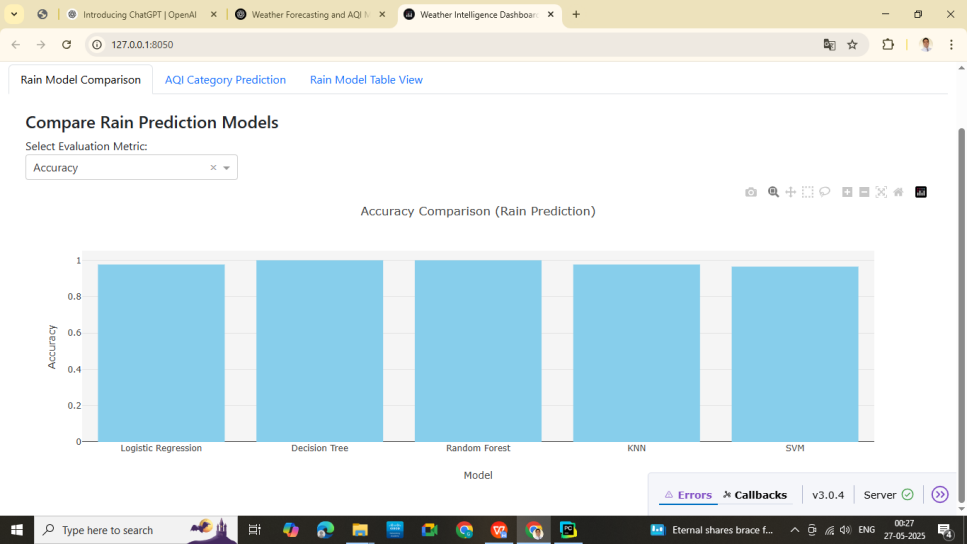
\includegraphics[width=\columnwidth]{image_6.png}
\caption{Rainfall Prediction Model Comparison Dashboard}
\label{fig:compare_dashboard}
\end{figure}

\begin{figure}[!t]
\centering
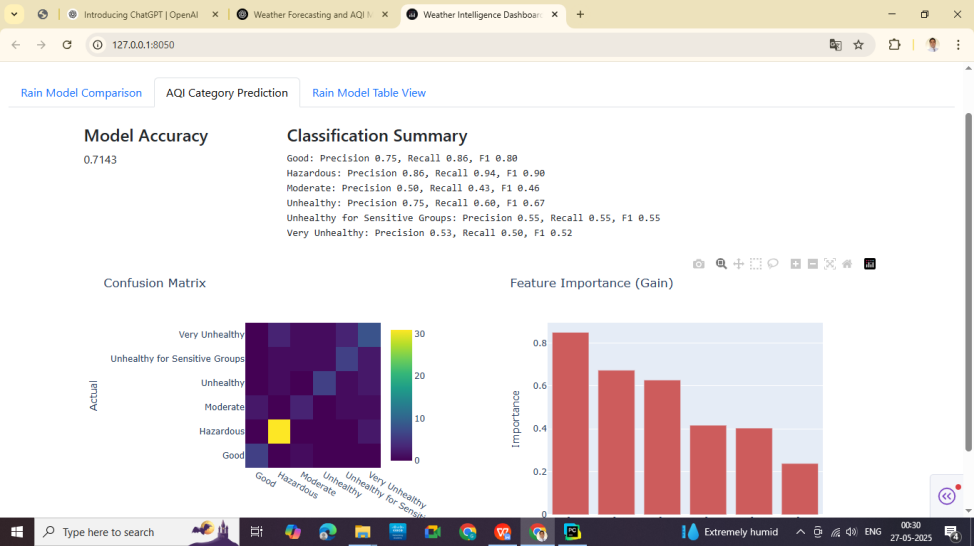
\includegraphics[width=\columnwidth]{image_7.png}
\caption{AQI Category Prediction Dashboard}
\label{fig:aqi_dashboard}
\end{figure}

\begin{figure}[!t]
\centering
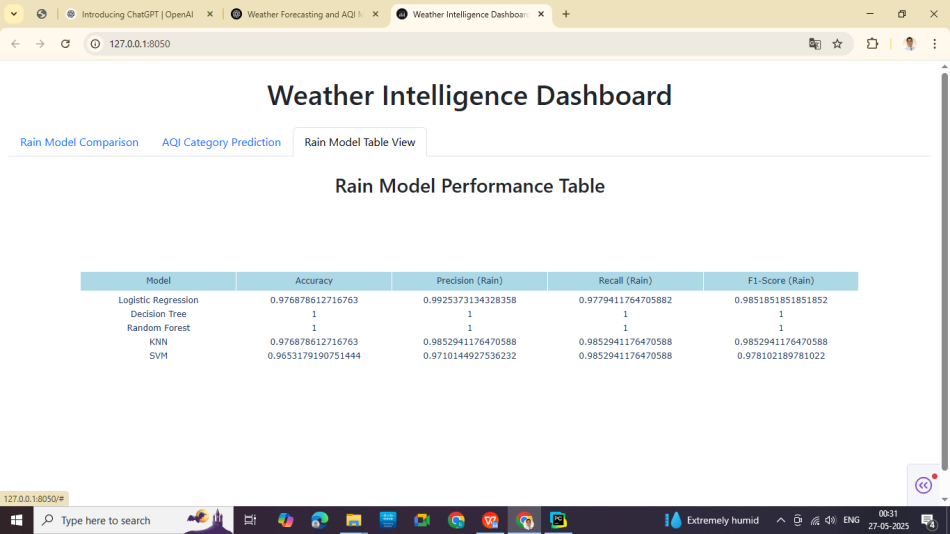
\includegraphics[width=\columnwidth]{image_8.png}
\caption{Rainfall Prediction Performance Dashboard}
\label{fig:rain_dashboard}
\end{figure}

Feature importance analysis identified humidity and atmospheric pressure as key contributors to rainfall prediction. The integration of Power BI dashboards and a Flask-based web application enables effective visualization, analysis, and decision support, making the proposed framework suitable for applications in agriculture, environmental monitoring, urban planning, and smart city development.

\section{Conclusion and Future Scope}

This paper presented an IoT-based weather monitoring and prediction framework that integrates environmental sensors, ThingSpeak cloud services, machine learning models, Flask-based visualization, and Power BI dashboards. The experimental results demonstrated strong predictive performance, with Random Forest achieving an $R^2$ score of 0.94 for temperature forecasting, XGBoost achieving a precision of 71.43\% for AQI classification, and Random Forest and Decision Tree classifiers achieving a precision of 100\% for rainfall prediction. The proposed framework provides a scalable and cost-effective solution for real-time environmental monitoring and forecasting, making it suitable for applications in smart cities, agriculture, and environmental management. Future work will focus on edge-based model deployment, integration of deep learning techniques such as LSTM, incorporation of satellite and GIS data, and expansion toward large-scale smart-city monitoring systems.

\begin{thebibliography}{99}

\bibitem{ref1}
A. Sharma, R. Gupta, and P. Singh,
``Deep learning-based weather prediction using LSTM and GRU networks,''
\textit{Journal of Environmental Informatics},
vol. 45, no. 2, pp. 123--135, 2024.

\bibitem{ref2}
M. Khan, S. Ali, and T. Rahman,
``IoT-driven real-time weather monitoring and forecasting mobile application,''
\textit{Sustainable Computing: Informatics and Systems},
vol. 39, pp. 100--112, 2025.

\bibitem{ref3}
R. Patel, K. Mehta, and S. Joshi,
``Integrated IoT-based weather monitoring and machine learning prediction system,''
\textit{International Journal for Research in Applied Science and Engineering Technology (IJRASET)},
vol. 13, no. 1, pp. 245--252, 2025.

\bibitem{ref4}
S. Verma and A. Kulkarni,
``IoT-based environmental monitoring system with machine learning approaches: A review,''
\textit{International Journal of Advanced Computer Science and Applications},
vol. 15, no. 3, pp. 210--220, 2024.

\bibitem{ref5}
Y. Zhang, L. Wang, and H. Chen,
``Hyperlocal weather prediction and anomaly detection using IoT and machine learning,''
\textit{arXiv preprint arXiv:2310.11001},
2023.

\bibitem{ref6}
P. Reddy and V. Kumar,
``Real-time IoT-based weather monitoring system using cloud platforms,''
\textit{International Journal of Engineering Research \& Technology (IJERT)},
vol. 13, no. 5, pp. 78--84, 2024.

\bibitem{ref7}
J. Singh and R. Kaur,
``Machine learning techniques for rainfall prediction: A comparative study,''
\textit{Procedia Computer Science},
vol. 218, pp. 456--463, 2023.

\bibitem{ref8}
H. Liu, X. Zhao, and Y. Sun,
``Air quality prediction using hybrid deep learning models,''
\textit{Scientific Reports},
vol. 14, no. 1, pp. 1--12, 2024.

\bibitem{ref9}
D. Roy and S. Banerjee,
``Support vector regression for short-term weather forecasting,''
in \textit{Proc. International Conference on Emerging Technologies},
2025, pp. 89--95.

\bibitem{ref10}
T. Dang, T. Tran, K. Nguyen, T. Pham, N. Pham, T. Vu, and P. Nguyen,
``ioTree: A battery-free wearable system with biocompatible sensors for continuous tree health monitoring,''
in \textit{Proc. 28th Annual International Conference on Mobile Computing and Networking (MobiCom)},
Sydney, NSW, Australia, Oct. 17--21, 2022, pp. 769--771.

\end{thebibliography}

\section*{Acknowledgement}

The authors thank the Department of Computer Science and Engineering, Government College of Engineering and Leather Technology, Kolkata, India, for providing academic support and laboratory facilities for conducting this research.

\section*{Author Biographies}

\noindent\textit{Abbreviations: B.Tech.--Bachelor of Technology, M.Tech.--Master of Technology, M.S.--Master of Science in Engineering, CSE--Computer Science and Engineering, GCELT--Government College of Engineering and Leather Technology, IIT--Indian Institute of Technology, IISc--Indian Institute of Science, NITTTR--National Institute of Technical Teachers' Training and Research.}

\vspace{0.5em}

\textbf{Nayan Saha} received his B.Tech. degree in CSE from GCELT, Kolkata, India. His research interests include IoT, AI, environmental monitoring, weather prediction, cloud computing, and smart consumer technologies.

\vspace{0.5em}

\textbf{Banibrata Manna} received his B.Tech. degree in CSE from GCELT, Kolkata, India. His research interests include deep learning and computer vision. He is currently pursuing an M.S. by Research in Intelligent Systems in the Department of CSE at IIT Bombay, India.

\vspace{0.5em}

\textbf{Mrinmayee Maity} received her B.Tech. degree in CSE from GCELT, Kolkata, India. Her research interests include AI, machine learning, cloud computing, data analytics, and smart IoT-enabled systems. She is currently pursuing an M.Tech. in CSE at IISc Bengaluru, India.

\vspace{0.5em}

\textbf{Sunayani Mondal} received her B.Tech. degree in CSE from GCELT, India. Her research interests include data science, machine learning, environmental informatics, and smart sensing technologies. She is currently pursuing an M.Tech. in CSE at NITTTR Kolkata, India.

\vspace{0.5em}

\textbf{Chhotan Mal} is a faculty member in the Department of CSE, GCELT, Kolkata, India. His research interests include machine learning, intelligent systems, data analytics, and IoT-enabled applications.

\vspace{0.5em}

\textbf{Debayan Ganguly} is a faculty member in the Department of CSE, GCELT, Kolkata, India. His research interests include machine learning, intelligent systems, data analytics, and IoT-enabled applications.

\end{document}